\section{问题二的模型建立与求解}

\subsection{因果滚动预测}

在日期 $d$ 的 0:00，分别以最近 1 日同区间值、近 7 日均值和最近 4 个同星期均值构造三个基预测器 $\widehat y^{(j)}_{d,t}$。以此前最近 14 个完整日期上的 MAE 倒数确定权重：
\begin{equation}
\omega_{j,d}=\frac{(\mathrm{MAE}_{j,d}+\varepsilon)^{-1}}
{\sum_{k=1}^{3}(\mathrm{MAE}_{k,d}+\varepsilon)^{-1}},\qquad
\widehat y_{d,t}=\sum_{j=1}^{3}\omega_{j,d}\widehat y^{(j)}_{d,t}.
\end{equation}
该过程对负载和光伏分别执行。正式回测期的负载预测 MAE、RMSE 和 WAPE 分别为
$45.1495~\mathrm{kWh}$、$62.6314~\mathrm{kWh}$ 和 $5.8677\%$；光伏对应指标为
$27.2149~\mathrm{kWh}$、$52.8739~\mathrm{kWh}$ 和 $6.8642\%$。

\subsection{安全裕度与日前计划}

设净负荷预测残差为
$e_{d,t}=(L_{d,t}-G_{d,t})-(\widehat L_{d,t}-\widehat G_{d,t})$。
对过去 28 日的同区间残差取分位数得到安全裕度 $q_{d,t}$。在 1 月历史上按时间顺序比较
$0.70,0.75,0.80,0.85,0.90$ 五个候选值，并以过购损失加 5 倍欠购损失作为验证准则，最终选择 0.75 分位数。

日前计划仍满足式~(\ref{eq:soc})和式~(\ref{eq:balance})，其中需求改为
$\widehat L_{d,t}+q_{d,t}$。问题二至四不在日末重置 SOC，而将实际日末状态传给次日；有限时域目标中加入基于次日边际电价的终端电量价值，防止日末系统性放空。

\subsection{逐段实际执行}

计划 $x_{d,t}$ 确定后，区间 $t$ 到来时才读取该区间的实际 $L_{d,t}$ 和 $G_{d,t}$。
若计划购电与光伏有富余，则优先满足负载、再充电，最后弃光；若有缺口，则在 SOC 和功率允许范围内放电，剩余缺口为
\begin{equation}
u_{d,t}=\max\left\{0,L_{d,t}-x_{d,t}-G_{d,t}-r_{d,t}\right\}.
\end{equation}
总费用为 $C_2=\sum p_tx_{d,t}+5\sum p_tu_{d,t}$。

\subsection{全年结果}

334 天的计划费为 $1335.33$ 万元，紧急购电费为 $172.80$ 万元，总费用为
$1508.13$ 万元；紧急购电量为 $27.80$ 万 $\mathrm{kWh}$。四个代表日结果见表~\ref{tab:p2days}。

\begin{table}[H]
\centering
\caption{问题二代表日结果}
\label{tab:p2days}
\begin{tabular}{lrrrr}
\toprule
日期 & 计划购电/kWh & 计划费/元 & 紧急费/元 & 总费用/元 \\
\midrule
3 月 20 日 & 68228.65 & 41419.24 & 759.50 & 42178.75 \\
6 月 21 日 & 43866.18 & 25669.21 & 0.00 & 25669.21 \\
9 月 23 日 & 67409.25 & 41781.55 & 3781.12 & 45562.67 \\
12 月 21 日 & 88870.34 & 55595.29 & 28915.03 & 84510.32 \\
\bottomrule
\end{tabular}
\end{table}

\begin{figure}[H]
  \centering
  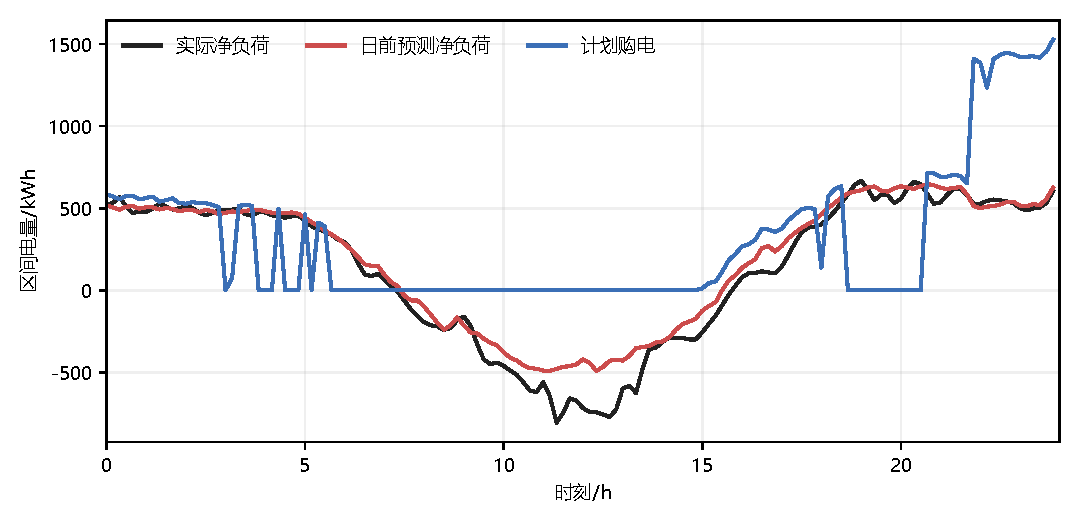
\includegraphics[width=0.9\textwidth]{../figures/p2_forecast_dispatch.pdf}
  \caption{6 月 21 日的净负荷预测与计划购电}
  \label{fig:p2forecast}
\end{figure}

\begin{figure}[H]
  \centering
  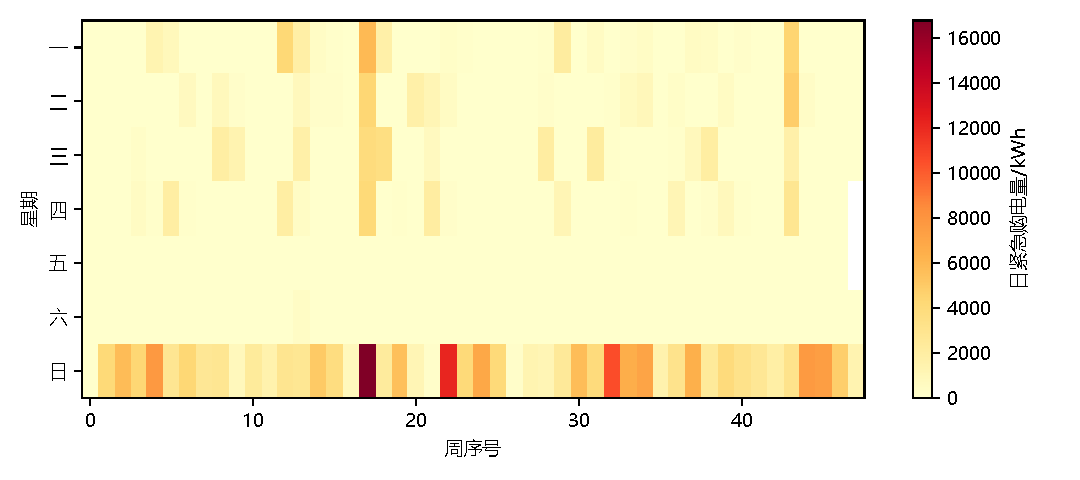
\includegraphics[width=0.9\textwidth]{../figures/p2_emergency_heatmap.pdf}
  \caption{问题二全年紧急购电量的周内分布}
  \label{fig:p2emergency}
\end{figure}
